% Compile this figure with XeLaTeX. All artwork is drawn with TikZ.
\documentclass[tikz,border=1pt]{standalone}
\usepackage{fontspec}
\setmainfont{Times New Roman}
\usetikzlibrary{arrows.meta}
\definecolor{ink}{HTML}{203944}
\definecolor{muted}{HTML}{52656E}
\definecolor{hair}{HTML}{AAB8BA}
\definecolor{panelrule}{HTML}{CAD5D6}
\definecolor{ocean}{HTML}{236D70}
\definecolor{indigo}{HTML}{535F90}
\definecolor{clay}{HTML}{965136}
\definecolor{seaWash}{HTML}{EDF5F3}
\definecolor{euWash}{HTML}{F2F2F8}
\definecolor{briWash}{HTML}{FAF3ED}
\definecolor{seaLight}{HTML}{B9DCD5}
\definecolor{pale}{HTML}{E7F0EE}
\tikzset{
  every node/.style={inner sep=0pt,outer sep=0pt,text=ink},
  heading/.style={font=\fontsize{13}{14}\selectfont\bfseries,anchor=west},
  subheading/.style={font=\fontsize{10.9}{12}\selectfont\bfseries,anchor=west},
  body/.style={font=\fontsize{9.2}{10.2}\selectfont,anchor=west},
  scope/.style={font=\fontsize{8.8}{9.5}\selectfont\itshape,anchor=west,text=muted},
  portname/.style={font=\fontsize{8.5}{9}\selectfont,text=ink,inner sep=0pt},
  route/.style={line width=1.12pt,line cap=round},
  otherroute/.style={draw=hair,line width=.75pt,dash pattern=on 1.8pt off 1.6pt,line cap=round},
  branch/.style={draw=muted,line width=.62pt,line cap=round,line join=round},
  icon/.style={line width=.85pt,line join=round,line cap=round}
}
% Reusable vector symbols. Coordinates are local to the enclosing scope.
\newcommand{\shipicon}{%
  \draw[icon] (-6.8,-1.5)--(6.8,-1.5)--(4.7,-4.2)--(-4.8,-4.2)--cycle;
  \draw[icon] (-5.8,-1.4)--(-5.8,1.1)--(-2.8,1.1)--(-2.8,-1.4)
    (-5.1,1.2)--(-5.1,3.4)--(-3.25,3.4)--(-3.25,1.2);
  \foreach \x in {-1.9,.65,3.2}{\draw[icon] (\x,-1.4) rectangle ++(2.15,2.05);}
  \foreach \x in {-1.9,.65}{\draw[icon] (\x,.7) rectangle ++(2.15,1.7);}
  \draw[icon] (-6.8,-5.75)..controls(-4.7,-4.8)and(-3.3,-6.7)..(-1.5,-5.75)
    ..controls(.2,-4.9)and(1.8,-6.6)..(3.5,-5.75)..controls(4.7,-5.2)and(5.8,-5.5)..(6.5,-5.65);
}
\newcommand{\globeicon}{%
  \draw[icon] (0,0) circle (2.65);
  \draw[icon] (0,0) ellipse (1.15 and 2.65) (-2.6,0)--(2.6,0);
}
\newcommand{\euring}{%
  \foreach \i in {0,...,11}{
    \fill ({2.35*cos(30*\i+90)},{2.35*sin(30*\i+90)}) circle (.35);
  }
}
\newcommand{\craneicon}{%
  \draw[icon] (-2.4,-2.5)--(-.1,-2.5) (-1.6,-2.45)--(-1.6,2.4)--(2.6,1.2)--(-2.55,1.2)
    (-1.6,-.9)--(-.7,.8) (1.95,1.13)--(1.95,-.65)
    (1.3,-.75) rectangle (2.55,-1.65);
}
\newcommand{\scaleicon}{%
  \draw[icon] (0,-4.6)--(0,3.4) (-2.7,-4.7)--(2.7,-4.7)
    (-5.6,1.6)--(0,2.6)--(5.6,1.6);
  \fill (0,3.4) circle (.62);
  \foreach \x in {-4.75,4.75}{
    \draw[icon] (\x,1.65)--++(-1.75,-3.25) --++(3.5,0)--cycle;
    \draw[icon] (\x-1.75,-1.65)..controls(\x-1.2,-3.05)and(\x+1.2,-3.05)..(\x+1.75,-1.65);
  }
}
% The four nodes and five edges are identical in each schematic.
\newcommand{\routes}[3]{% accent, list of credited edges, list of eligible sites
  \coordinate (E) at (-17,.25); \coordinate (N) at (-5,6.4);
  \coordinate (B) at (1.8,-3.5); \coordinate (C) at (15.3,2.75);
  \foreach \u/\v in {E/N,E/B,N/B,N/C,B/C}{\draw[otherroute] (\u)--(\v);}
  \foreach \u/\v in {#2}{\draw[route,draw=#1] (\u)--(\v);}
  \foreach \p in {E,N,B,C}{\filldraw[fill=white,draw=muted,line width=.8pt] (\p) circle (1.13);}
  \foreach \p in {#3}{\filldraw[fill=#1,draw=#1,line width=.7pt] (\p) circle (1.13);}
  \node[portname,anchor=north] at (-17,-1.25) {EU};
  \node[portname,anchor=south] at (-5,7.85) {Other};
  \node[portname,anchor=north] at (1.8,-5.05) {BRI};
  \node[portname,anchor=south] at (15.3,4.2) {BRI};
}
\newcommand{\plan}[8]{% x, accent, ground, icon, title, edges, sites, rule text
  \begin{scope}[shift={(#1,0)}]
    \fill[#3,rounded corners=1.3mm] (0,36.6) rectangle (49.6,77.8);
    \draw[#2,line width=1.25pt,line cap=round] (2,76.9)--(47.6,76.9);
    \begin{scope}[shift={(6,71.65)},color=#2]#4\end{scope}
    \node[subheading,text=#2] at (11.55,71.65) {#5};
    \begin{scope}[shift={(24.85,55.8)}]\routes{#2}{#6}{#7}\end{scope}
    \draw[#2!28!white,line width=.45pt] (3,46)--(46.6,46);
    #8
  \end{scope}
}
\newcommand{\ruletext}[2]{%
  \node[scope] at (3.2,42.9) {Routes}; \node[body] at (14,42.9) {#1};
  \node[scope] at (3.2,38.75) {Sites}; \node[body] at (14,38.75) {#2};}
\begin{document}
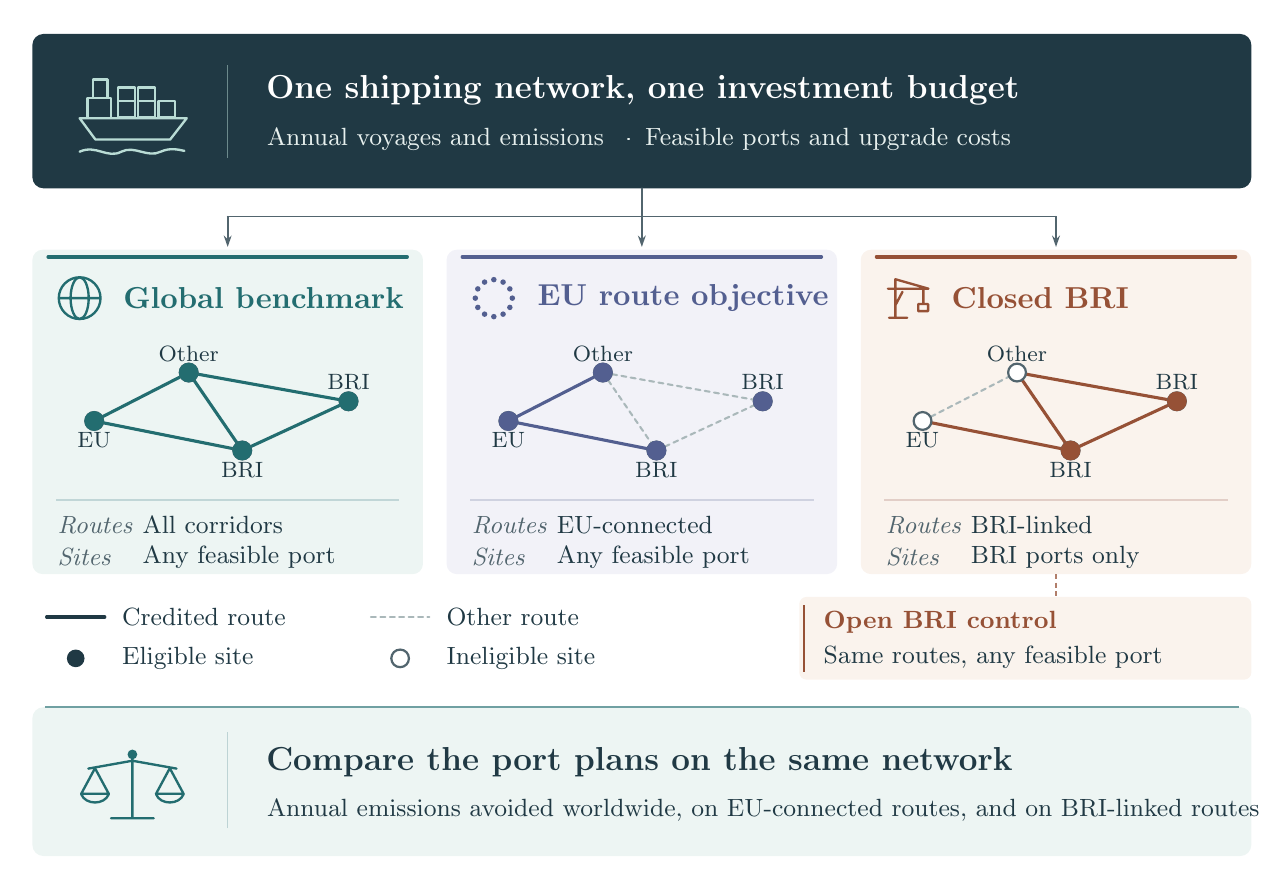
\begin{tikzpicture}[x=1mm,y=1mm]
  \path[use as bounding box] (0,0) rectangle (156,106);
  \fill[ink,rounded corners=1.4mm] (0.6,85.6) rectangle (155.4,105.2);
  \begin{scope}[shift={(13.4,96)},color=seaLight]\shipicon\end{scope}
  \draw[seaLight!50!ink,line width=.55pt] (25.4,89.5)--(25.4,101.2);
  \node[heading,text=white] at (30.3,98.0) {One shipping network, one investment budget};
  \node[body,text=pale] at (30.4,91.8) {Annual voyages and emissions \enspace·\enspace Feasible ports and upgrade costs};
  \draw[branch] (78,85.6)--(78,82) (25.4,82)--(130.6,82);
  \foreach \x in {25.4,78,130.6}{\draw[branch,-{Stealth[length=1.45mm,width=1.0mm]}] (\x,82)--(\x,78.15);}
  \plan{.6}{ocean}{seaWash}{\globeicon}{Global benchmark}
    {E/N,E/B,N/B,N/C,B/C}{E,N,B,C}{\ruletext{All corridors}{Any feasible port}}
  \plan{53.2}{indigo}{euWash}{\euring}{EU route objective}
    {E/N,E/B}{E,N,B,C}{\ruletext{EU-connected}{Any feasible port}}
  \plan{105.8}{clay}{briWash}{\craneicon}{Closed BRI}
    {E/B,N/B,N/C,B/C}{B,C}{\ruletext{BRI-linked}{BRI ports only}}
  % Legend and the single changed assumption in the open-domain control.
  \draw[route,draw=ink] (2.4,31.15)--(9.8,31.15);
  \node[body] at (12,31.15) {Credited route};
  \draw[otherroute] (43.6,31.15)--(51,31.15);
  \node[body] at (53.2,31.15) {Other route};
  \fill[ink] (6.1,25.9) circle (1.12);
  \node[body] at (12,25.9) {Eligible site};
  \filldraw[fill=white,draw=muted,line width=.8pt] (47.3,25.9) circle (1.12);
  \node[body] at (53.2,25.9) {Ineligible site};
  \draw[clay!74,line width=.7pt,dash pattern=on 1.8pt off 1.25pt] (130.6,36.6)--(130.6,33.7);
  \fill[briWash,rounded corners=.9mm] (98.0,23.2) rectangle (155.4,33.7);
  \draw[clay,line width=1pt] (98.6,24.2)--(98.6,32.7);
  \node[subheading,text=clay,font=\bfseries\fontsize{9.4}{10}\selectfont] at (101.1,30.5) {Open BRI control};
  \node[body] at (101.1,26.0) {Same routes, any feasible port};
  \fill[seaWash,rounded corners=1.4mm] (.6,.8) rectangle (155.4,19.7);
  \draw[ocean!65,line width=.7pt] (2.2,19.7)--(153.8,19.7);
  \begin{scope}[shift={(13.3,10.3)},color=ocean]\scaleicon\end{scope}
  \draw[ocean!30,line width=.55pt] (25.4,4.35)--(25.4,16.55);
  \node[heading] at (30.3,12.7) {Compare the port plans on the same network};
  \node[body] at (30.4,6.6) {Annual emissions avoided worldwide, on EU-connected routes, and on BRI-linked routes};
\end{tikzpicture}
\end{document}

